\subsection{Einleitung}
Der Zeeman-Effekt beschreibt die Aufspaltung und Polarisation von Spektrallinien eines Atoms unter dem Einfluss eines äußeren Magnetfeldes.
Durch das Aufspalten der diskreten Energieniveaus kommt es bei der Lichtemission zu kleinen Unterschieden in der Wellenlänge gegenüber der Emission im feldfreien Fall.

\paragraph{Magnetisches Moment}
Hüllenelektronen können mit dem Bahndrehimpuls $\vec{l}$ und mit dem Eigendrehimpuls $\vec{s}$ beschrieben werden.
Dabei gilt:
\begin{align*}
  |\vec{l}|=\sqrt{l(l+1)}\hbar&& \text{mit } l &= 0,1,2,...,n-1\\
  |\vec{s}|=\sqrt{s(s+1)}\hbar&& \text{mit } s &= \frac{1}{2}.
\end{align*}
Die magnetischen Momente, welche durch die Drehimpulse und die Ladung der Elektronen entstehen, können beschrieben werden mit:
\begin{align*}
  \vec{\mu}_l &= -\mu_B \frac{\vec{l}}{\hbar} = -\mu_B \sqrt{l(l+1)}\vec{l}_e\\
  \vec{\mu}_s &= -g_S \frac{\mu_B}{\hbar}\vec{s} = -g_S \mu_B \sqrt{s(s+1)}\vec{s}_e.\\
\end{align*}
$\vec{l}_e$ und $\vec{s}_e$ sind die Einheitsvektoren in die jeweiligen Richungen $l$ und $s$. \textbf{\huge{HIER}}
Die Größe $g_S$ ist der Landé-Faktor. $\mu_B$ beschreibt das Bohrsche Magneton und ist dabei gegeben als:
\begin{align*}
  -\frac{1}{2} e_0 \frac{\hbar}{m_0}.
\end{align*}
Weiter gilt, dass $e_0$ die Elementarladung und $m_0$ die Elektronenmasse beschreibt.

\subsection{Wechselwirkung der Drehimpulse und magnetischer Momente untereinander}
Für Atome mit mehreren Elektronen gibt es viele unterschiedliche Arten, wie Bahndrehimpuls und Spin miteinander wechselwirken können.
Im Wesentlichen können zwei einfache Grenzfälle betrachtet werden, welche häufig in der Natur vorkommen.
%
Für Atome mit niedriger Kernladungszahl kann der Gesamtbahndrehimpuls $\vec{L}$ der Hülle aus den Bahndrehimpulsen $\vec{l}$ vektoriell zusammengesetzt werden.
Das liegt an der großen Wechselwirkung zwischen den Bahndrehimpulsen.
\begin{align*}
  \vec{L} = \sum_i{\vec{l}_i} \text{ mit } |\vec{L}|= \sqrt{L(L+1)}\hbar
\end{align*}
Für den Gesamtbahndrehimpuls müssen nur unabgeschlossene Schalen betrachtet werden, da abgschlossene Schalen immer einen Bahndrehimpuls von 0 besitzen.
$\vec{l}$ kann dabei nur ganzzahlige Quantenzahlen von 0,1,2 oder 3 annehmen.
Je nach Quantenzahl kann zwischen S,P,D und F-Term unterschieden werden.
Das magnetische Moment $\vec{\mu}_L$ vom Gesamtbahndrehimpuls $\vec{L}$ lässt sich errechnen mit:
\begin{align*}
  |\vec{\mu}_L| = \mu_B\sqrt{L(L+1)}.
\end{align*}
%
Für den Gesamtspin der Elektronenhülle $\vec{S}$ gilt für Atome mit niedriger Ordnungszahl ebenfalls die vektorielle Summation der einzelnen Komponenten.
Die Einzelkomponenten sind hier die Einzelspins $\vec{s}_i$.
\begin{align*}
  \vec{S} = \sum_{i}{\vec{s}_i}
\end{align*}
Die Gesamtspinquantenzahl $S$ kann die Werte $\frac{N}{2}, \frac{N}{2}-1, ..., \frac{1}{2},0$ annehmen.
$N$ beschreibt dabei die Anzahl der Elektronen aus den unabgeschlossenen Schalen.
Der Betrag des Gesamtspins lässt sich aufstellen zu:
\begin{align*}
  |\vec{S}| = \sqrt{S(S+1)}\hbar.
\end{align*}
Der dazugehörige Betrag des magnetischen Momentes ist gegeben als:
\begin{align*}
  |\vec{\mu}_S| = g_S\mu_B\sqrt{S(S+1)}.
\end{align*}
Im Falle, dass das Atom keinem zu großen Magnetfeld ausgesetzt ist kann der Gesamtdrehimpuls $\vec{J}$ geschrieben werden als:
\begin{align*}
  \vec{J} = \vec{L}+ \vec{S}.
\end{align*}
Die beschriebene LS-Kopplung ist für die Betrachtung des Zeeman-Effekts zugrunde gelegt.
$\vec{J}$ kann abhängig von $S$ ganz- oder halbzahlig sein.
Der Betrag vom Gesamtdrehimpuls ist gegeben als:
\begin{align*}
  |\vec{J}| = \sqrt{J(J+1)}\hbar.
\end{align*}
Beschreibt man ein Energienivau, kann das mit der Darstellung
\begin{align*}
  {}^M\mathcal{L}_J
\end{align*}
erfolgen.
$M$ ist dabei die Multiplizität und von $S$ abhängig in der Form $M=2S+1$.
Für das Bahndrehimpulssymbol $\mathcal{L}$ gilt:
$\mathcal{L}\in\{S(L=0), P(L=1), D(L=2), F(L=3)\}$.
Wobei $L$ wieder der Gesamtdrehimpuls ist.\\
%
Der zweite Grenzfall betrachtet die j-j-Kopplung bei Atomen mit höheren Kernladungszahlen.
Durch die starke Kopplung zwischen dem Spin und dem Bahndrehimpuls eines Einzelelektrons setzt sich der Gesamtdrehimpuls des Elektrons nun zusammen aus:
\begin{align}
  \vec{j}_i = \vec{l}_i + \vec{s}_i.
  \label{eqn.j}
\end{align}
Der Gesamtdrehimpuls der Elektronenhülle lässt sich schreiben als:
\begin{align*}
  \vec{J}=\sum_i\vec{j}_i.
\end{align*}
Da sich wie in Formel \ref{eqn.j} beschrieben $\vec{j}_i$ aus $\vec{l}_i$ und $\vec{s}_i$ zusammensetzt kann bei dieser Betrachtung kein Gesamtdrehimpuls $\vec{L}$ oder ein Gesamtspin $\vec{S}$ definiert werden.
\textbf{\huge{Es kann bei dieser Betrachtung kein Gesamtdrehimpuls $\vec{L}$ oder ein Gesamtspin $\vec{S}$ definiert werden.}}\\
Für Atome mit mittlerer Kernladungszahl besteht ein fließender Übergang zwischen den beiden Grenzfällen.
\FloatBarrier

\subsection{Energieaufspaltung und Übergänge}
%
\begin{figure}[h!]
  \centering
  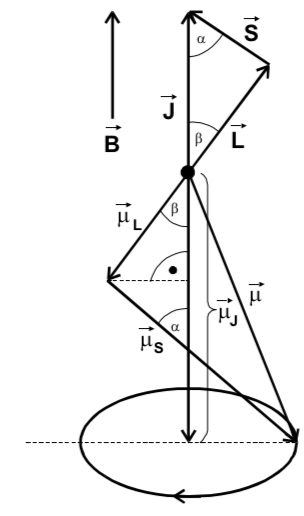
\includegraphics[width=5cm]{magmom1.png}
  \caption{Darstellung der verschiedenen magnetischen Momente von Spin, Bahndrehimpuls und Gesamtdrehimpuls}
  \label{fig:mag}
\end{figure}
%
Das magnetische Moment, welches zum Gesamtdrehimpuls $\vec{J}$ gehört, lässt sich berechnen mit
\begin{align*}
  \vec{\mu}_J&=\mu_Bg_J\sqrt{J(J+1)},
\end{align*}
wobei für den Landé-Faktor $g_J$ des entsprechenden Atoms gilt:
\begin{align}
		g_J:=&\frac{3J(J+1)+S(S+1)-L(L+1)}{2J(J+1)}.
\end{align}
\FloatBarrier

Durch die Richtungsquantelung sind nur genau $2J+1$ Einstellungen des atomaren magnetischen Momentes zu der äußeren Feldrichtung möglich.
Die zusätzliche Energie, die das Moment $\vec{\mu}$ im äußeren Magntfeld bekommt, ist gegeben als:
\begin{align*}
  E_{\text{mag}} = -\vec{\mu}_J \cdot \vec{B} = mg_J\mu_B B.
\end{align*}
Für die Orientierungsquantenzahl $m$ gilt $-J < m < J$.
Für den Fall, dass $B \ne 0$ spaltet sich also das Enaginiveau $E_0$ eines Atoms auf in $2J+1$ äquidistante Niveaus.
%In der Abbildung %\ref{fig.J2}
%ist diese Aufspaltung für $J = 2$ abgebildet.
%\begin{figure}[h!]
%	\centering
%	\includegraphics[width=0.6\textwidth]{Aufspaltung.pdf}
%	\caption{Aufspaltung eines Energieniveaus von einem Atom mit $J=2$. \cite{V27}}\label{fig:J2}
%\end{figure}
Diese Aufspaltung der Spektrallinien unter einem angelegten Magnetfeld wird als Zeeman-Effekt bezeichnet.

Die Auswahlregeln beschreiben die möglichen Energieübergänge.

Für die Festlegung der Auswahlregeln wird die zeitabhängige Schrödingergleichung benötigt.
\begin{align}
	-\frac{\hbar^2}{2m}\Delta \psi(\vec{r},t)+U\psi(\vec{r},t)-i\hbar\frac{\partial \psi(\vec{r},t)}{\partial t}=0.
\end{align}
\textbf{\huge{HIER: Wie und warum setzt sich $\psi$ aus mehreren Wellenfunktionen zusammen?}}
Die Lösung $\psi$ beschreibt den Übergang zwischen den Energieniveaus $\alpha$ und $\beta$.
Aus der Lösung ergibt sich eine Schwingung des Elektrons mit der Frequenz:
\begin{align*}
  \nu_{\alpha\beta}:=\frac{E_\alpha-E_\beta}{h}.
\end{align*}
Das schwingende Elektron lässt sich dementsprechend als Dipol beschreiben.
Das Dipolmoment in die x-Richtung sieht wie folgt aus:
\begin{align*}
  	D_x=-e_0\text{const } 2 \Re \real\left( \underbrace{\int x\psi^*_\beta\psi_\alpha dV}_{x_{\alpha\beta}}\exp(2\pi i\nu_{\alpha,\beta}t) \right).
\end{align*}
Für die $y$- und $z$-Richtung kann die Formel analog aufgestellt werden.
Das Integal $x_{\alpha\beta}$ und seine analogen $y$- und $z$-Komponenten werden als Matrixelemente bezeichnet und sind wichtig für die Berechnung des Poynting-Vektors $\vec{S}_{\alpha\beta}$.
Der Poyning-Vektor berechnet sich nach:
\begin{align*}
  |\vec{S}_{\alpha\beta}| \sim \left(|x_{\alpha\beta}|^2+|y_{\alpha\beta}|^2+|z_{\alpha\beta}|^2\right) \text{sin}^2(\gamma).
\end{align*}
$\gamma$ beschreibt dabei den Winkel zwischen Dipolmoment und Ausbreitungsrichtung der Strahlung.
Es kann gezeigt werden, dass die Intensität der vom Dipol emittierten Strahlung mit den Matixelementen zusammenhängt.
Für den Fall, dass das B-Feld in die Z-Richtung zeigt, verschwindet $z_{\alpha\beta}$, außer wenn gilt, dass $m_{\alpha} = m_{\beta}$.
$x_{\alpha\beta}\pm i y_{\alpha\beta}$ verschwindet ebenfalls, außer wenn gilt, dass $m{\beta} = m_{\alpha} \pm 1$.
Zum Zeeman-Effekt kommt es also nur, wenn sich die Orientierungsquantenzahlen $m_{\alpha}$ und $m_{\beta}$ gar nicht oder nur um $\pm 1$ unterscheiden.\\
%
Für den Fall, dass $\Delta m = 0$ ($z_{\alpha\beta} \neq 0,\ x_{\alpha\beta} = i y_{\alpha\beta} = 0$)ist, kommt es zur Schwingung des Dipols parallel zur Magnetfeldachse.
Dies führt bei der Emission zu linear-polarisiertem Licht parallel zu $\vec{B}$.
Durch die Polarisation kann das emittierte Licht am besten senkrecht (transversal) zur Feldrichtung beobachtet werden.
Die Strahlungsart wird als $\pi$ bezeichnet.\\
%
Für den Fall, dass $\Delta m = \pm 1$ ($z_{\alpha\beta} = 0,\ x_{\alpha\beta} = \pm i y_{\alpha\beta} \neq 0$) ist, kommt es zu links oder rechts zirkular-polarisierter Stahlung um die Magnetfeldachse.
Bei Betrachtung transversal zur Feldachse erscheint das emittierte Licht linear polarisiert und senkrecht zu $\vec{B}$.
Die Strahlungsarten werden als $\sigma$ bezeichnet.
%
Die oben getroffenen Aussagen gelten nur für den Fall, dass $S=0$ ist.
Diesen Spezialfall bezeichnet man als normalen Zeeman-Effekt.
Für Übergänge mit $S=0$ gilt $g_J = 1$.
Die Verschiebung der Energieniveaus ist dementsprechend unabhängig von den Quantenzahlen.
Der Energieunterschied $\Delta E$ zwischen den Niveaus ist unabhängig von $L$ und $J$ gleich groß.
\begin{align}
  \Delta E = m \mu_B B \text{ für } -J \leq m \leq J
  \label{eqn:normal}
\end{align}

Der anormale Zeeman-Effekt kommt deutlich häufiger vor und tritt auf, wenn $S \neq 0$ ist.
Es gelten für die Übergänge die selben Auswahlregeln $\Delta m = 0, \pm 1$.
Da $g_J = 1$ nicht mehr gegeben ist, ergeben sich für die Übergänge die Energien von:
\begin{align}
	E &=& (m_ig_{J_i}-m_jg_{J_j})\mu_BB+E_0
  \label{eqn:anormal}\\
    &=& g_{ij}\mu_BB + E_0.
    \label{eqn:allgemein}
\end{align}
Dabei ist $g_{ij}$ der Landé-Faktor des Übergangs.
\FloatBarrier

\subsection{Vorbereitungsaufgabe}
\begin{figure}[h!]
  \centering
  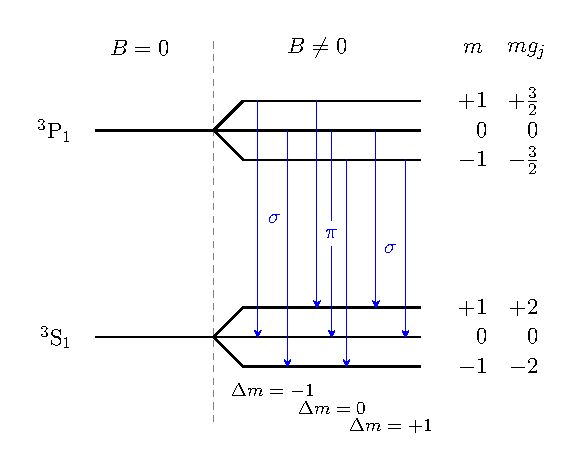
\includegraphics[width=9cm]{termschema_blau.pdf}
  \caption{Termschema eines ${}^3P_1\leftrightarrow {}^3S_1$ Übergangs. Der Übergang liegt im blauen Wellenlängenbereich.}
  \label{fig:blau}
\end{figure}
\begin{figure}[h!]
  \centering
  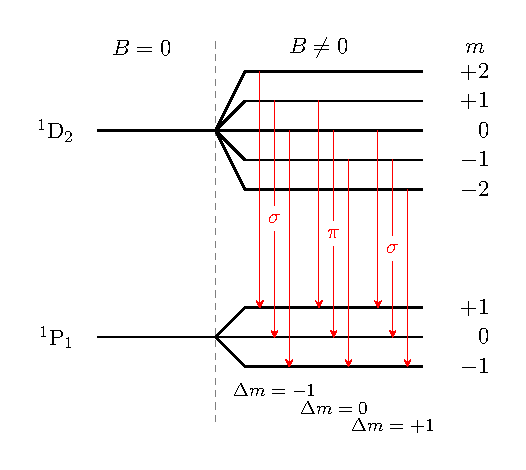
\includegraphics[width=9cm]{termschema_rot.pdf}
  \caption{Termschema eines ${}^1D_2 \leftrightarrow {}^1P_1$ Übergangs. Der Übergang liegt im roten Wellenlängenbereich.}
  \label{fig:rot}
\end{figure}
\FloatBarrier
\begin{table}
	\centering
	\begin{tabular}{cccccc}
		\toprule
		Übergang & $m_1$  & $g_{1}$ & $m_2$ & $ g_2$ & $g_{12}$\\
		\midrule
		& \multicolumn{2}{c}{${}^1P_1$}  & \multicolumn{2}{c}{${}^1D_2$} \\
		\midrule
		& 2 & 1 & 1 & 1 & 1\\
		$\sigma$& 1 & 1 & 0 & 1 & 1\\
		& 0 & 1 & -1 & 1 & 1\\
		\midrule
		& 1 & 1 & 1 & 1 & 0\\
		$\pi$ & 0 & 1 & 0 & 1 & 0\\
		& -1 & 1 & -1 & 1 & 0\\
		\midrule
		& 0 & 1 & 1 & 1 & -1\\
		$\sigma$ & -1 & 1 & 0 & 1 & -1\\
		& -2 & 1 & -1 & 1 & -1\\\bottomrule
	\end{tabular}
	\caption{Hier sind die Landé-Faktoren der roten Spektrallinie aufgeführt.}
	\label{tab:Lande_rot}
\end{table}
\begin{table}
	\centering
	\begin{tabular}{cccccc}
		\toprule
		Übergang & $m_1$  & $g_{1}$ & $m_2$ & $ g_2$ & $g_{12}$\\
		\midrule
		& \multicolumn{2}{c}{${}^3S_1$}  & \multicolumn{2}{c}{${}^3P_2$} \\
		\midrule
		$\sigma$ & +1 & 2 & 0 & $\frac{3}{2}$& 2\\
		& 0 & 2 & -1 & $\frac{3}{2}$ & $\frac{3}{2}$\\
		\midrule
		& +1 & 2 & +1 & $\frac{3}{2}$ & $\frac{1}{2}$\\
		$\pi$ & 2 & 2 & 0 & $\frac{3}{2}$ & 0 \\
		& -1 & 2 & -1 & $\frac{3}{2}$ & -$\frac{1}{2}$\\
		\midrule
		& 0 & 2 & 1 & $\frac{3}{2}$ & -$\frac{3}{2}$\\
		$\sigma$ & -1 & 2 & 0 & $\frac{3}{2}$& -2\\
		\bottomrule
	\end{tabular}
	\caption{Hier sind die Landé-Faktoren der blauen Spektrallinie aufgeführt.}
	\label{tab:Lande_blau}
\end{table}
\FloatBarrier
